%%%%%%%%%%%%%%%%%%%%%%%%%%%%%%%%%%%%%%%%%%%%%%%%%%%%%%%%%%%%%%%%%%%%%%%%
\chapter{Einleitung}
\label{sec:introduction}
%%%%%%%%%%%%%%%%%%%%%%%%%%%%%%%%%%%%%%%%%%%%%%%%%%%%%%%%%%%%%%%%%%%%%%%%

%=======================================================================
\section{Problemstellung}
%=======================================================================
Einer der größten Trends auf den Business-Markt ist die Mobilisierung der Geschäftswelt, die sich in den verschiedensten Unternehmensstrategien widerspiegelt. Es gibt zahlreiche Innovationen, um unabhängig von Stakeholdern, Zeit, Ort und Geräten auf Daten und Anwendungen zuzugreifen. Ein wesentlicher Innovationsstrang ist dabei die Entwicklung von Business-Apps, um beispielsweise die Arbeitszeiten auf Geschäftsreisen effektiv ausnützen zu können. Dadurch hat die Bedeutung der Informations- und Kommunikationsindustrie in den letzten Jahren in den Unternehmen stetig zugenommen \cite{smartMobileApps1}.
\\\\
Durch die immer stärkere Nachfrage nach mobilen Apps im Arbeitsalltag ist es notwendig, mobile Endgräte in bestehende Geschäftsprozesse der Unternehmen zu integrieren. Dabei soll es vermieden werden, eine komplett neue IT-Infrastruktur unter Beteiligung von mobilen Endgeräten zu schaffen. In vielen Unternehmen wird daher die IT-Anwendungslandschaft an das Paradigma der serviceorientierten Architektur ausgerichtet. Ein wesentlicher Vorteil dabei ist, dass wohl definierte Schnittstellen vorhanden sind und angebotene Dienste flexibel und plattformunabhängig genutzt werden können. Sollen nur mobile Anwendungen in die existierende IT-Anwendungslandschaft eingegliedert werden, bedeutet dies in der serviceorientierten Architektur, das Web Services benötigt werden. In der Praxis werden Web Services entweder mit dem Kommunikationsprotokoll \acrfull{SOAP} oder \acrfull{REST} umgesetzt \cite{smartMobileApps17}.
\\\\
Im Revex2020 Projekt wird das Kommunikationsprotokoll REST verwendet, dadurch ist es nötig ein geeignetes Framework aufseiten der mobilen App zu finden, dass eine vollständige und korrekte Anbindung an den Webservice ermöglicht. Es existieren bereits zahlreiche Frameworks, die eine REST Implementierung unterstützen, diese unterscheiden sich aber stark in der Qualität und im Funktionsumfang. Auch bieten nicht alle diese Frameworks eine Unterstützung für Android an. Daher ist die Auswahl eines geeigneten Frameworks für eine erfolgreiche Implementierung ausschlaggebend. 

%=======================================================================
\section{Motivation}
%=======================================================================

Die Thematik rund um REST-Frameworks für Android ist noch relativ neu, dadurch ist es nicht möglich ohne größere Recherchen ein geeignetes Framework für das Projekt Revex2020 auszuwählen. Es gibt zwar einige Vergleiche von REST Frameworks, wie etwa die Fachstudie von Markus Fischer, Kalman Kepes und Alexander Wassiljew \cite{vergleich13}. In dieser Studie wird allerdings nicht darauf eingegangen, ob die Frameworks eine Implementierung clientseitig mit Android unterstützen, es wird die vermehrt auf die serverseitige Implementierung eingegangen. Die Möglichkeit der clientseitigen Implementierung ist aber eine essenzielle Anforderung, da eine Business-App für Android entwickelt werden soll. 
\\\\
Der immer stärker wachsende Bereich von mobilen Anwendungen macht das zu untersuchende Thema besonders interessant. Herkömmliche Software rückt immer weiter in den Hintergrund, Daten sollen sofort und überall abgerufen werden können. Mobile Endgeräte wie Smartphone und Tablets verändern daher die Geschäftswelt nachhaltig, Führungskräfte und Mitarbeiter erhalten jederzeit Zugang zu Unternehmensinformationen und -prozessen. Die Unternehmen der Zukunft werden daher mobil \cite{smartMobileApps7}.  
\\\\
Revex2020 ist ein Forschungsprojekt zur Revitalisierung von Wasserkraftwerken, das in Kooperation mit dem Institut für Energietechnik und Thermodynamik entwickelt wird \cite{doujak}. Ein Ziel dieses Projektes ist es, Mitarbeitern zukünftig zu ermöglichen, mithilfe von mobilen Endgeräten den Zustand einzelner Kraftwerkskomponenten vor Ort erfassen zu können. Es soll eine Android-App entwickelt werden, die das bereits vorhandene Backend, über das REST-Webservices nutzt um exemplarisch den Anwendungsfall abzubilden.

%=======================================================================
\section{Zielsetzung}
%=======================================================================

Ziel dieser Bachelorarbeit ist die Evaluierung verschiedener REST-Frameworks für Android im Kontext des Revex2020 Projekts, um eine unkomplizierte Anbindung an das bereits vorhandene Backend zu ermöglichen. Dazu werden bestehende REST-Frameworks für Android getestet, indem diese in einem Anwendungsfall eingesetzt werden. Nach der Evaluierung dieser Frameworks soll eine Empfehlung abgegeben werden, welches sich am besten für das Revex2020 Projekt eignet.
\\\\
Die Evaluierung der Frameworks erfolgt anhand von Prototypen, indem die REST-Frameworks verwendet werden. Es wurden im Vorfeld verschiedene Anwendungsfälle definiert (siehe Abbildung \ref{figure:useCase}), indem die einzelnen REST Frameworks integriert werden. Dabei werden in einem Szenario verschiedene Prozesse durchgespielt, wie Kraftwerk erstellen, löschen, bearbeiten und anzeigen. Als Vorlage dazu wurde die bestehende Web-Applikation des Projektes verwendet.
\\\\

\begin{minipage}{\textwidth} 
	\centering	
	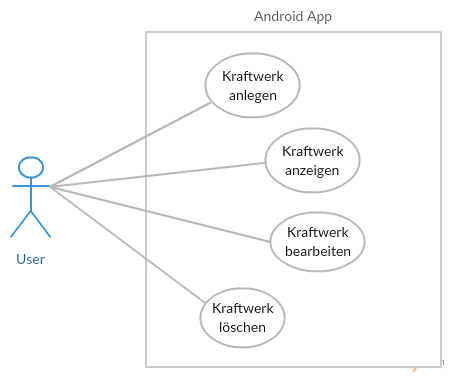
\includegraphics[width=0.65\textwidth]{figures/kraftwerke_use_case.png}
	\captionof{figure}{Use-Case-Diagramm}
	\label{figure:useCase}
	\vspace{2ex}
\end{minipage}

%=======================================================================
\section{Methodik}
\label{sec:methodik}
%=======================================================================
Die Qualität der einzelnen Frameworks soll anhand folgender Kriterien verglichen werden, welche an dem Kriterienkatalog der Fachstudie "Vergleich von Frameworks zur Implementierung von REST-basierten Anwendungen" \cite{vergleich13} angelehnt sind. Dieser Kriterienkatalog beschäftigt sich mit den Eigenschaften für die Evaluierung von REST Frameworks, vor allem auf serverseitiger Sicht. Der Kriterienkatalog wurde deshalb gekürzt bzw. einzelne Punkte zusammengefasst und abgeändert, um eine Evaluierung im Kontext des Projektes Revex2020 durchführen zu können. 
\\\\
Das Hauptaugenmerk der Evaluierung liegt auf der Clientseite, da die entwickelte App eine Client Applikation darstellt. Deswegen wurden spezifische Kriterien der Fachstudie zu einer REST Server Applikation gestrichen. Beispielsweise wurde der gesamte Kriterienblock über Ressourcentypen \cite{ressourcen:rest} weggelassen, da es für die clientseitige Verarbeitung irrelevant ist, welche Ressourcentypen serverseitig implementiert werden können. 
\\\\
\textbf{Allgemein:}
\begin{itemize}
	\item Existiert eine aktive Community?
	\item Ist eine Dokumentation des Codes vorhanden? (Schnittstellenbeschreibung, JavaDoc)
	\item Unter welcher Lizenz steht das Projekt zur Verfügung?
	\item Gibt es Hilfestellung für Entwicklung? (Tutorial, Codebeispiele)
\end{itemize}

\textbf{Implementierung mit REST-Framework:}
\begin{itemize}
	\item Wie lange wird benötigt um das Framework einzubinden?  (Zeitdauer)
	\item Welche \acrfull{HTTP}-Verben werden unterstützt? (GET, POST, PUT, DELETE etc.)
	\item Gibt es Möglichkeiten den HTTP-Header zu verändern oder zu erweitern?
	\item Welche Medientypen werden unterstützt? (JSON, HTML, XML etc.)
	\item Wie erfolgt die Identifikation einzelner Ressourcen? (Aufruf der URL)
	\item Wird das HATEOAS Konzept unterstützt?
\end{itemize}

\textbf{Erweiterte Technische Fähigkeiten}
\begin{itemize}
	\item Definiert das Framework eine eigene IDL\footnote{Schnittstellenbeschreibungssprachen}?
	\item Wie wird der Bereich Sicherheit gehandhabt?  (Authentifizierung, Verschlüsselung)
	\item Werden andere Protokolle außer HTTP noch unterstützt?
	\item Gibt es eine Möglichkeit für asynchronen Nachrichtenaustausch?
	\item Wird transaktionales Verhalten vom Framework unterstützt? (ACID-Eigenschaften)
\end{itemize}

